%\documentclass[]{article}
\documentclass[]{../../../../tex/classes/homework}
\usepackage{../../../../tex/packages/hebrewSupport}
\usepackage{../../../../tex/packages/mathShortcuts}
%\usepackage{../../../../tex/packages/theoremsSupport}

\usepackage{pgfplots}
\usepgfplotslibrary{fillbetween}
\usepackage{nicematrix}

%\usepackage{multicol}
%
%
%%% Math packages
%\RequirePackage{ifxetex,ifluatex,amssymb,amsmath,mathrsfs,amsthm,witharrows,mathtools,mathdots,centernot}
%\RequirePackage{amsmath}
%\renewcommand{\qedsymbol}{$\blacksquare$} % end proofs with \blacksquare. Overwrites the defualts.
%\RequirePackage{bm}
%
%% Design
%\RequirePackage[margin=1in]{geometry}
%\RequirePackage[skip=4pt, indent=0pt]{parskip}
%\RequirePackage[normalem]{ulem}
%\renewcommand\labelitemi{$\bullet$}
%
%
%\newcommand\ff{\mathrm{f}}
%\newcommand\gcc{G^{\mathrm{SCC}}}
%\newcommand\squigT{\overset{T}{\squig}}
%\newcommand\squigd{\leftrightsquigarrow}
%\DeclareMathOperator{\low}{low}
%\DeclareMathOperator{\sol}{sol}
%\DeclareMathOperator{\val}{val}
%\DeclareMathOperator{\key}{key}
%\DeclareMathOperator{\Left}{left}
%\DeclareMathOperator{\Right}{right}
%
%\setlength{\parindent}{0pt}
%\setlength{\parskip}{4pt}



\DeclareMathOperator*{\argmin}{arg\,min}
\newcommand\I  {(\mathrm{I})}
\newcommand\II {(\mathrm{II})}

\newcommand\qq  {(\mathrm{1})}
\newcommand\ww  {(\mathrm{2})}
\newcommand\ee  {(\mathrm{3})}
\newcommand\rr  {(\mathrm{4})}

\author{שחר פרץ}
\title{אלגוריתמים $\sim$ \textit{תרגיל בית 5}}
\begin{document}
	\maketitle
	
%	\ {} \\ \ \\ \ \\ 
	\section{}
	נתונות $n$ נקודות שונות במישור $(x_1, y_1) \dots (x_n, y_n)$. נרצה לצייר $n$ עיגולים גדולים ככה האפשר במישור כך ש־$(x_i, y_i)$ היא מרכזו של עיגול ה־$i$. מותר לעיגולים להשיק. נקודה תהיה עיגול מנוון. 
	
	\begin{enumerate}[(A)]
		\item \textbf{הבעיה הרגילה: }נחפש $n$ משתנים ממשיים $r_1 \dots r_n$, שיהיו הרדיוסים שלנו. 
		\begin{itemize}
			\item \textbf{פונקציית מטרה: }
			\[ \bm{\max f(r_1, ..., r_n) = \max\sum^{n}_{i = 1}r_i} \]
			נכונות נובעת ישירות מהגדרת סכום היקפים מקסימלי. 
			\item \textbf{אילוצים לינאריים: }התנאי ששני עיגולים ישיקו אך לא יחתכו/יכילו אחד את השני, שקול לכך שכל שני עיגולים $i, j \in [n]$ יקיימו את התנאי: 
			\[ d((x_i, y_i), (x_j, y_j)) \ge r_i + r_j \]
			מהגדרת עיגול. נכניס את הגדרת פונקציית המרחק ונקבל $\frac{n^{2} - n}{2}$ אילוצים לינאריים: 
			\[ \forall i, j \in \{1 \dots n\} \co \quad \bm{\sqrt{(x_i - x_j)^{2}+ (y_i - y_j)^{2}} \ge r_i + r_j} \]
			(נבחין שהאילוץ לינארי שכן המקדמים של $r_i, r_j$ קבועים). 
			נוסף על כך, רדיוס צריך להיות מספר אי־שלילי. לכן נוסיף עוד $n$ אילוצים: 
			\[ \bm{r_i \ge 0} \]
			(נבחין שזו הצורה הסטנדרטית, שכן כל המשתנים אי־שליליים)
		\end{itemize}
		\item \textbf{הבעיה הדואלית: }נחפש $m = \frac{n^{2} - n}{2}$ משתנים (כי $n$ האילוצים האחרונים נתונים מהצורה הסטנדרטית) ו־$n$ א''שים. נגדיר משתנים $y_{11} \dots y_{nn}$ (כאשר $y_{ij} = y_{ji}$). 
		\begin{itemize}
			\item \textbf{פונקציית מטרה: }
			\[ \min f = \min b^{T}y = \bm{\min \csb{\ \sum_{\mathclap{i, j = 1}}^{n}y_{ij}\sqrt{(x_j - x_i)^{2} + (y_j - y_i)^{2}} }} \]
			\item \textbf{אילוצים: }נבחין ש־$c = (1, 1 \dots 1)$ ונוציא את השורות הרלוונטיות ב־$A$ למציאת $n$ אילוצים: 
			\[ \forall i \in \{1 \dots n\}\co \quad\quad \bm{\sum_{\mathclap{i \neq j = 1}}^{n}y_{ij} \ge 1} \]
			כאשר כמובן כל המשתנים אי־שליליים ($y_{ij} \ge 0$). 
		\end{itemize}
		זאת כי המטריצה של הבעיה המקורית היא: 
		\[ (A)_{(\ml, k),i} = \begin{cases}
			1 & i = \ml \oplus i = k \\
			0 & \other
		\end{cases} \]
		(כאשר $\oplus$ זה xor) ורק נותר לקחת לה transpose כדי למצוא את האילוצים לעיל. 
	\end{enumerate}
	
%	\newpage \ \newpage 
	\npage
	
	\section{}
	נתונה מערכת משוואות לינארית עם $m$ משוואות ו־$n$ נעלמים המוגדרת ע''י המטריצה $A \in \R^{m \times n}$ ווקטור $b \in \R^{m}$. נאמר ש־$x \in \R^{n}$ הוא פתרון $\eg$־מקורב אם $\norm{Ax - b}_1 = \eg$. נמצא פתרון $\eg$־מקורב עבור $\eg$ מינימלי. 
	
	\textbf{סימונים: }$x = (x_1 \dots x_n)$, $b = (b_1 \dots b_m)$ וכן $A = (a_{ij})_{i \in [m], j \in [n]}$. 
	
	נבחין ששקול לפתור את הבעיה תחת האילוץ (הלכאורה חלש יותר) ש־$\sof{Ax - b}_1 \le \eg$, כמו שראינו בתרגול. נגדיר את $\eg_1 \dots \eg_n$ ו־$x_1 \dots x_n$ להיות המשתנים של התוכנית, כאשר בהקשר של הבעיה המקורית נדרוש ש־$\eg_i \ge \sof{(Ax - b)_i}$ (לכן $\eg \le \sum_{i = 1}^{n} \eg_i$). 
	\begin{itemize}
		\item \textbf{פונקציית מטרה: }
		\[ \min \sum_{i = 1}^{n}\eg_i \]
		\item \textbf{אילוצים: }נדרוש ש־$\sof{Ax - b}_1 \le \eg$. נבחין ש־: (לכל $i \in [n]$)
			\begin{align*}
				& \eg_i \ge \sof{(Ax - b)_i} = \sof{-b_i + \sum_{j = 1}^{n}a_{ji}x_j} \\
				\iff & \begin{cases}
					&\disty {\eg_i \ge -b_i + \sum_{j = 1}^{n}a_{ji}x_j} \\
					\land & \disty {\eg_i \ge b_i - \sum_{j = 1}^{n}a_{ji}x_j}
				\end{cases} \iff \begin{cases}
					&\disty \bm{b_i \ge -\eg_i+ \sum_{j = 1}^{n}a_{ji}x_j} \\
					\land & \disty \bm{b_i \ge \eg_i + \sum_{j = 1}^{n}a_{ji}x_j}
				\end{cases}
			\end{align*}
			כאשר $x_1 \dots x_n \in \R$, ו־$\eg_1 \dots \eg_n \in \R_{\ge0}$ כי הם משקלים, כלומר: 
			\[ \forall i \in [n] \co \quad \quad \bm{\eg_i \ge 0} \]
		\item \textbf{שקילות לבעיה המקורית: }נבחין ש־: 
		\[ \eg = \norm{Ax - b}_1 \!= \sum_{i= 1}^{n}\sof{(Ax - b)_i} \le \sum_{i =1}^{n}\eg_i \]
		נתבונן ב־$x$ ה־$\eg$־מקורב המינימלי. במצב זה נוכל לבחור את הפתרון $\eg_i = -b_i + \sum_{j = 1}^{n}a{ji}x_j$ ואז נקבל התלכדות של השוויונות לעיל. סה''כ בעבור $x$ מינימלי הפותר את הבעיה הסכום אכן יתלכד עם הפתרון. עוד נבחין שהבעיה שכן השווינות מתקיים בעבור $x = 0$, $\eg_i = b_i$. 
	\end{itemize}
%	נגדיר את $x_1 \dots x_n$ להיות המשתנים שלנו. 
%	\begin{itemize}
%		\item \textbf{פונקציית מטרה: }נרצה ש־$\eg$ יהיה המינימלי. אנו פועלים תחת האילוץ ש־$\norm{Ax - b}_1 \le \eg$, לכן באופן שקול נוכל לדרוש ש־$\norm{Ax - b}_1$ יהיה מינימלי. נמצא נוסחה סגורה: 
%		\begin{align*}
%			\norm{Ax - b}_1 &= \sum_{i = 1}^{n}\sof{(Ax - b)_i} \\
%			&= \sum_{i = 1}^{m}\sof{-b_i + \sum_{j = 1}^{n}a_{ji}x_j} = \sum_{i = 1}^{m}\sof{\,\sum_{j = 1}^{n}\cl{a_{ji}x_j - \frac{b_i}{n}}} = \sum_{j = 1}^{n}\sum_{i = 1}^{m}\sof{a_{ji}x_j - \frac{b_i}{n}}
%		\end{align*}
%	\end{itemize}
	
%	\newpage \ \newpage
	\npage
	\section{}
	נתון גרף לא מכוון $G = (V, E)$. 
	
	\begin{enumerate}[(A)]
		\item \textbf{שאלה: }נאמר שפונקציית משקל $w \co V \to [0, 1]$ \textit{מקליקה} אם לכל $\{u, v\}\notin E$ מתקיים $w(u) + w(v) \le 1$. נמצא פונקציית משקל מקליקה שממקסמת את סכום משקלי הצמתים. 
		
		\textbf{תשובה: }נגדיר את $w_1 \dots w_n$ (כאשר $n = \sof V$) להיות הצמתים (כאשר את $\sof V$ נמספר $v_1 \dots v_n$). 
		\begin{itemize}
			\item \textbf{פונקציית מטרה: }
			\[ \bm{\max \sum_{i =1}^{n}w_i} \doc \sof{w} \]
			\item \textbf{אילוצים: }אילוץ השאלה: 
			\begin{align*}
				\forall i, j \ \mathrm{s.t. }\ \{v_i, v_j\}\notin E\co \quad\quad &\bm{{w_i + w_j \le 1}} \\
			\end{align*}
			אילוץ המשקלים (אי־שליליים בתחום $[0, 1]$): 
			\begin{align*}
				\forall i \in [n]\co\quad\quad &w_i \le 1 \land w_i \ge 0 \\
				\iff &\begin{cases}
					\bm{w_i \le 1} \\
					w_i \ge 0
				\end{cases}
			\end{align*}
			כמובן שכל המשקלים אי־שליליים. 
			
			השקילות לבעיה המקורית די ברורה מאליה, שכן הניסוח של בעיית ה־LP לעיל הוא ניסוח פורמלי של המילים הכתובות בשאלה. סה''כ $m = \binom{n}{2}$ שוויונות (מתוכם $n$ הם מהצורה $w_i\le 1$ ו־$\frac{n^{2} - n}{2}$ מהצורה $w_j + w_i \le 1$, ו־$w_i \ge 0$ נתון מהצורה הסטנדרטית). 
			
			\item \textbf{מה בעיית ה־IP מייצגת: }אם נדרוש ש־$w \co V \to \{0, 1\}$, אז שהבעיה שקולה למציאת קליקה מקסימלית ($w(v) = 1$ אמ''מ הוא בקליקה). העובדה ש־$\range w = \{0, 1\}$ מאפשר לנו להגדיר ש''בחרנו`` צומת $v$ אמ''מ $w(v) = 1$. נוכיח שבחרנו את הצמתים שיוצרים את הקליקה המקסימלית בגרף. 
			\begin{itemize}
				\item \textbf{מקסימליות: }בהינתן קליקה $A$ פונקציות המשקל: 
				\[ w_A(v) = I_A(v) = \begin{cases}
					1 & v \in A \\
					0 & v \notin A
				\end{cases} \]
				בבירור מקיימת את האילוצים (אם $\{v_i, v_j\} \notin E$ אז לפחות אחד מהם בהכרח לא בקליקה, אחרת יש קשת בינהם. ולכן $w_A(i) + w_A(j) \le 1$) ו־$\sof w = \sof A$. לכן האופטימום חסום מלמטה ע''י הקליקה המקסימלית (שכן מצאנו פתרונות פיזביליים שבעבורם פונקציית המטרה הגודל של הקליקה). 
				\item \textbf{תקינות: }נוכיח שהצמתים שבחרנו (באופטימום) הם בהכרח קליקה. נסמן את קבוצת הצמתים שבחרנו ב־$C$. זה ברור מאליו שכן לכל זוג צמתים $v_i, v_j \in C$ שבחרנו, בהכרח $w_i + w_j = 2 \not \le 1$ ולכן $\{v_i, v_j\} \in E$ ולכן $C$ קליקה מהגדרה. 
			\end{itemize}
			סה''כ האופטימום משרה קליקה (תקינות) שחסומה מלמטה ע''י הקליקה המקסימלית (מקסימליות), ולכן הוא הקליקה המקסימלית, וסיימנו. 
		\end{itemize}
		
		
		
		\item \textbf{שאלה: }נסחו את הבעיה הדואלית. 
		
		\textbf{פתרון: }נבחין שבשאלה לעיל $w_i \ge 0$ וכן השוויונות מנוסחים בצורה הסטנדרטית. לכן השאלה לעיל מנוסחת בצורה הסטנדרטית. נגדיר מיפוי מזוגות (לא סדורים) של $V$ ל־$\{\ml, k\}$ לצורך הנוחות. 
		ננסח את השאלה לעיל במובנים של אלגברה לינארית: 
		\begin{align*}
			c &\in \R^{n} & c &= (1, 1 \dots 1) \\
			b &\in \R^{m} & b &= (1, 1 \dots 1) \\
			w &\in \R^{n} & w &= (w_1 \dots w_n) \\
			A &\in M_{m \times n}(\R) & (A)_{(\ml, k),i} &= \begin{cases}
				1 & (i = \ml \lor i = k) \land (v_k, v_\ml) \notin E \\
				0 & \other
			\end{cases}
		\end{align*}
		(נבחין שייתכן $\ml = m$) 	ואז הבעיה הפרימרית היא מהצורה $\max c^T x$ כך ש־$Aw \le b$ ו־$w \ge 0$. 
		
		כדי לנסח את הבעיה הדואלית, נגדיר משתנים $x_1 \dots x_{m}$ שיוכלו להיות ממופים גם הם ל־$x_1 \dots x_{k, \ml}$ (משום שאנו מדברים על קבוצה מגודל $\binom{n}{2}$, אז $x_{i,j} = x_{j,i}$). הבעיה הדואלית היא מהצורה $b^Tx$ כך ש־$x \ge 0$ וכן $A^Tx \ge c$. מהגדרת $A$, נבחין שהקורדינאטה ה־$j \in [n]$ ב־$A^Tx$ היא: 
		\[ (A^{T}x)_j = \sum_{i = 1}^{m}(A^{T})_{ji} \cdot x_i = \sum_{\mathclap{\{k, \ml\} \in \ps_2([n])}}(A)_{(\ml, k), j} \cdot x_{\ml, k} = \sum_{i = 1}^{n}x_{j, i} \cdot \begin{cases}
			1 & (v_i, v_j) \in E \\
			0 & (v_i, v_j) \notin E
		\end{cases} \]
		\begin{itemize}
			\item \textbf{פונקציית מטרה: }בבעיה הדואלית מנסים למצוא את $\min b^T x$. במקרה זה: 
			\[ \bm{\min \sum_{i =1}^{m}x_i} \]
			\item \textbf{אילוצים: }בבעיה הדואלית דורשים ש־$x \ge 0$ וכן $A^Tx \ge c$. כלומר: ($\adj v$ קבוצת השכנים של $v$)
			\[ \forall i \in [n] \co \quad\quad \bm{1\le \sum_{\mathclap{v_i \notin \adj(v_j)}}^{n}x_{j, i}} \]
			וכן: 
			\[ \forall i, j \in [n] \co \quad\quad \bm{x_{ij} \ge 0} \]
			\item \textbf{מה בעיית ה־IP} (של הדואל) \textbf{מייצגת: }אינני יודע. אשמח אם יתפרסם פתרון או אם הבודק יוכל לתת הסבר קצר. 
		\end{itemize}
	\end{enumerate}
	
%	\newpage 
	\npage
	
	\section{}
	נתונה קבוצה $S = \{1, 2 \dots n\}$ ו־$m$ ת''קים $A_1 \dots A_m \subset S$. 
	\begin{enumerate}[(A)]
		\item נגדיר \textit{קבוצה מכסה שברית} כפונקציה $f \co S \to \R_{\ge 0}$ כך שלכל $i \in [m]$ מתקיים $\sum_{j \in A_i}f(j) \ge 1$. נסמן $\sof f \cod \sum_{j \in S}f(j)$, ונכתוב LP כך ש־$\sof f$ מינימלי. 
		
		נגדיר משתנים $f_1 \dots f_n$ כך ש־$f_i = f(i)$. 
		\begin{itemize}
			\item \textbf{פונקציית מטרה: }
			\[ \min \sof f = \min \sum_{j \in S} f(j) = \bm{\min \sum_{i \in S}f_i} = \max\cl{\sum_{i \in S}- f_i} \]
			\item \textbf{אילוצים: }לכל $i \in [m]$ נגדיר את האילוץ: 
			\[ \sum_{j \in A_i}f(j) = \bm{\sum_{j \in A_i}f_j \ge 1} \iff \sum_{j \in A_i}-f_j \le -1 \]
			משום ש־$\range f = \R_{\ge 0}$, אז נדרוש גם $f_i \ge 0$ (שהמשתנים יהיו אי־שליליים). 
		\end{itemize}
		\item למציאת התוכנית הדואלית, נגדיר משתנים $x_1 \dots x_m$. 
		\begin{itemize}
			\item \textbf{פונקציית המטרה: }\[ \min \sum_{i = 1}^{n}(-1) \cdot x_i = \bm{\max \sum_{i = 1}^{n}x_i} \]
			\item \textbf{אילוצים: }נגדיר את האילוצים: 
			\begin{align*}
				\forall i \in [n] \co \quad\quad &\sum_{j = 1}^{m}-I_{A_j}(i)\cdot x_j \ge -1 \\
				\iff &  \sum_{j = 1}^{m}I_{A_j}(i) \cdot x_j \le 1
			\end{align*}
			כאשר $I_{A_j}$ האינדיקטור על $A_j$. 
			
			\textit{הערה: }נבחין שאם $A_1 \dots A_m$ איננו כיסוי של $S$, אז קיים $i \in [n]$ כך ש־$i \notin A_j$ לאף $j$, ואז הוא משרה אילוץ טאוטולוגי ($0 \le 1$) שנוכל להתעלם ממנו. כך נפעל לכל $i \in S = [n]$ ש־$A_1 \dots A_m$ לא מכסים. 
			\item \textbf{מה בעיית ה־IP מייצגת: }ראשית נשייך את האילוץ $x_j$ ל־$A_j$. 
			\begin{itemize}
				\item אם $A_j$ כלשהי ריקה, אז אין שום אילוץ על $x_j$ והבעיה לא חסומה. לכן מעתה ואילך נניח שאין קבוצה ריקה. 
				\item אחרת, $x_j \le 1$, שכן קיים אילוץ מהצורה $\cdots + 1 \cdot x_j + \cdots \le 1$ והמשקלים טבעיים. מכאן ש־$x_j \in \{0, 1\}$. 
				\item נאמר ש־$A_j$ \textit{נבחרה} אם $x_j = 1$ (יש לנו ''תירוץ`` להגדיר את זה תחת ההנחה שה־$A_j$־ים אינם ריקים, ואז $x_j$ הוא בינארי). 
				\item אם $A_{j_2} \cap A_{j_1} \neq \varnothing$, אז קיים $i \in A_{j_1} \cap A_{j_2}$ ואז הוא משרה אילוץ $x_{j_1} + x_{j_2} + \cdots \le 1$. מכאן שרק אחת מבין $A_{j_1}, A_{j_2}$ תיבחר. 
				\item סה''כ שתי קבוצות נבחרו אמ''מ אם הן זרות בזוגות. 
				\item נבחין ש־$\sum_{j = 1}^{n}x_i$ הוא מספר הקבוצות שנבחרו. 
			\end{itemize}
			סה''כ תוכנית ה־IP מוצאת את המספר המקסימלי של קבוצות זרות בזוגות (תחת הנחה שאף קבוצה אף אינה ריקה, שכן במקרה זה התוכנית לא חסומה). 
		\end{itemize}	
	\end{enumerate}
	
%	\newpage \ \newpage
	\npage
	\section{}
	\begin{enumerate}[(A)]
		\item נשרטט את הישרים של התוכנית, ונסמן את תחום הפיזביליות. 
		\begin{center}
			\sen 
			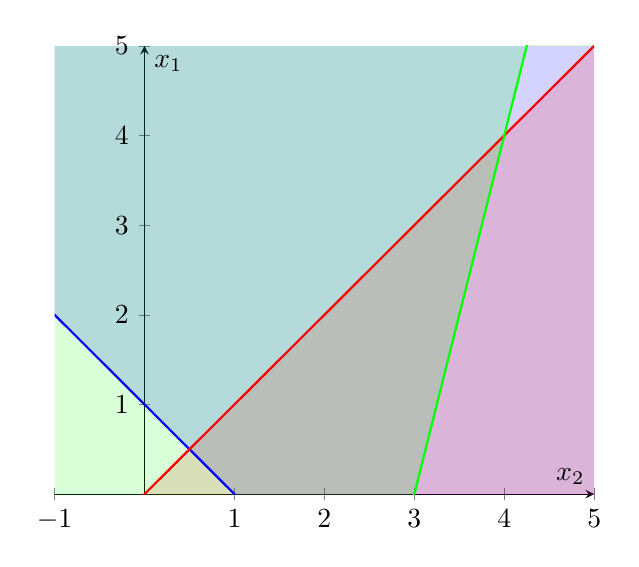
\begin{tikzpicture}
				\begin{axis}[
						axis lines = center,
						xlabel = $x_2$, ylabel = $x_1$,
						xmin = -1, xmax = 5,
						ymin = 0, ymax = 5
					]
					\addplot[name path=a1, thick, blue] {-x+1};
					\addplot[name path=a2, thick, red] {x};
					\addplot[name path=a3, thick, green] {4*x-12};
					\path[name path=baseline] (axis cs:-3,0) -- (axis cs:5,-3);
					\path[name path=upperline] (axis cs:-3,5) -- (axis cs:5,5);
					
					\addplot [fill=blue, fill opacity=0.17] fill between [
						of = a1 and upperline,
						soft clip = {domain=-3:5}
					];
					\addplot [fill=red, fill opacity=0.15] fill between [
						of = a2 and baseline,
						soft clip = {domain=-3:5}
					];
					\addplot [fill=green, fill opacity=0.15] fill between [
						of = a3 and upperline,
						soft clip = {domain=-3:5}
					];
%					\addplot[blue!20, opacity=0.5] fill between[
%					of = a1 and a2,
%					soft clip={domain=0:2}
%					];
				\end{axis}
			\end{tikzpicture}
			\she
		\end{center}
		כאשר שטח הפיזביליות הוא השטח האפור. ניתן לראות מהסרטוט שצורת ה־slack ההתחלתית (המצויה בראשית הצירים, שכן מציבים $x_ 1 = x_2 = 0$) אינה בתחום הפיזביליות. 
		\begin{center}
			\begin{multicols}{3}
				התחום הכחול: $-x_1-x_2 \le -1$ \\
				התחום האדום: $-x_1 + x_2 \le 0$ \\
				התחום הירוק: $4x_1  - x_2 \le 12$
			\end{multicols}
		\end{center}
		\item נמצא צורת slack פיזבילית עבורו $x_1 = 1 \land x_2 = 0$. בצורה ההתחלתית $x_2 = 0$ ולכן נעשה צעד pivot על $x_1$. לשם כך, ראשית נמיר את הבעיה לצורת Slack. נוסיף $x_3, x_4, x_5$ משתנים כנגד כל אחד מאי־השיוויונות. נקבל: 
		\[ \begin{alignedat}{9}
			\max &\quad 0 -x_1 + 2x_2 \\ 
			&\begin{cases}
				x_3 = &\dequad \ x_1 + x_2 - 1 \\
				x_4 = &\dequad \ x_1 - x_2 \\
				x_5 = &\dequad \ -4x_1 + x_1 + 12
			\end{cases}
		\end{alignedat} \]
		נחליף עם $x_3$ כדי לקבל החוצה משתנה חופשי $1$ (לאחר שנעביר אגפים ה־$-1$ החופשי של $x_3$ יהפוך להיות $x_1$ למעלה). ואז נקבל: 
		\[ \begin{alignedat}{9}
			\max &\quad 0 - (x_2 + x_3 + 1) &\quad \quad \implies\quad \quad  && \max &\quad -1 - x_3 + 3x_2 \\ 
			&\begin{cases}
				x_1 = &\dequad \ - x_2 + x_3 + 1 \\
				x_4 = &\dequad \ (-x_2 + x_3 + 1) - x_2 \\
				x_5 = &\dequad \ -4(-x_2 + x_3 + 1) + x_1 + 12
			\end{cases} &\quad \quad \implies\quad \quad  &&  \quad &\begin{cases}
				x_1 = &\dequad \ 1 - x_2 + x_3 \\
				x_4 = &\dequad \ 1 - 2x_2 + x_3 \\
				x_5 = &\dequad \ 8 + 5x_2 - 4x_3
			\end{cases}
		\end{alignedat}  \]
		עתה נבחין שבפתרון הבסיס של צורת ה־slack, שבו נציב במשתנים הלא־בסיסיים $x_3 = x_2 = 0$, נקבל שערך הפתרון $-1$ ו־$x_1 = 1$, כנדרש. 
		\item נחשב את ריצת הסימפלקס של התוכנית. ניעזר בצורת ה־slack הפיזבילית אליה הגענו בסעיף הקודם (חסכנו את השלב ההתחלתי באמצעות זה שסעיף ב' גילה לנו איך צעד pivot צריך לעשות כדי למצוא צורת slack פיזבילית). 
		\[ \begin{alignedat}{9}
			\max &\quad -1 - x_3 + 3x_2 &&& 
			\max &\quad \frac{1}{2} - \frac{3}{2x_4} + \frac{1}{2}x_2 &&&
			\max &\quad 4 - \frac{2}{3}x_4 - \frac{1}{3}x_5 \\ 
			&\begin{cases}
				x_1 = &\dequad \ 1 - x_2 + x_3 \\
				x_4 = &\dequad \ 1 - 2x_2 + x_3 \\
				x_5 = &\dequad \ 8 + 5x_2 - 4x_3
			\end{cases} &\quad \rrt{\mathrm{pivot}}{x_4 \to x_2}\quad &&&\begin{cases}
				x_1 = &\dequad \ \frac{1}{2} + \frac{1}{2}x_3 + \frac{1}{2}x_3 \\
				x_2 = &\dequad \ \frac{1}{2} + \frac{1}{2}x_3 - \frac{1}{2}x_4 \\
				x_5 = &\dequad \ 10\frac{1}{2} - 1\frac{1}{2}x_3 - 2\frac{1}{2}x_4
			\end{cases} &\quad \rrt{\mathrm{pivot}}{x_5 \to x_3}\quad &&&\begin{cases}
				x_1 = &\dequad \ 4 - \frac{2}{3}x_4 - \frac{1}{3}x_5 \\
				x_2 = &\dequad \ 4 - 1\frac{1}{3}x_4 - \frac{1}{3}x_5 \\
				x_3 = &\dequad \ 7 - 2\frac{1}{3}x_4 - \frac{2}{3}x_5
			\end{cases}
		\end{alignedat}  \]
		סה''כ נציב במשתנים הלא־בסיסיים אפסים ונקבל $x_1 = 3, x_2 = 4$ וערך פתרון מקסימלי $4$ (בדיקת שפיות: בהכרח נגיע לקצה של הפוליהדרון של סעיף (א) כשנגיע לאופטימום של הסימפלקס, מה שאכן קרה). 
	\end{enumerate}
	
%	\newpage \ \newpage
	\npage
	\section{}
	תהי $P$ תוכנית לינארית פיזבילית וחסומה בצורה סטנדרטית ו־$D$ הדואלית לה. נתון פתרון פרימאלי $\hat x$ ופתרון דואלי $\hat y$. ידוע שכל אחד מהם הוא פיזבילי. נוכיח כי הם אופטימליים אמ''מ: 
	\begin{align*}
		\I && \forall i &\in [m]\co & [A\hat x]_i \hat y_i   = \sum_{j= 1}^{n} a_{ij}\hat x_j \hat y_i = b_i \hat y_i = [b^Ty]_i \\
		\II&& \forall j &\in [n]\co & [A^T\hat y]_j \hat x_i = \sum_{i= 1}^{m} a_{ij}\hat y_j \hat x_i = c_i \hat x_i = [c^Tx]_i
	\end{align*}
	
	\begin{proof}
%		נבחין שנוכל לחלק את $\I$ ב־$\hat y_i$ ואת $\II$ ב־$\hat x_j$ כדי לקבל ביטוי שקול (עד לכדי חילוק באפס – זו לא בעיה כי בה''כ נוכל להזיז את הפוליהדרון למקום בו תחום הפיזביליות לא פוגש ב־$0$ המ''מ, פורמליזם בסוף): 
%		\begin{align*}
%			\I && \forall i &\in [m]\co & \sum_{j= 1}^{n} a_{ij}\hat x_j = b_i &&\iff&& Ax = b \\
%			\II&& \forall j &\in [n]\co & \sum_{i= 1}^{n} a_{ij}\hat y_i = c_i &&\iff&& A^{T}y = c
%		\end{align*}
		\begin{itemize}
			\item[$\implies$]תחת ההנחה שהשוויונות מתקיימים, נקבל ש־: 
			\begin{align*}
				b^Ty = \sum_{i = 1}^{m}b_i \hat y_i &\overset{\I}{=} \sum_{i = 1}^{m}\sum_{j= 1}^{n} a_{ij}\hat x_j \hat y_i \\
				&=\sum_{j = 1}^{n}\sum_{i = 1}^{m} a_{ij}\hat x_j \hat y_i 
				\overset{\II}{=}\sum_{j = 1}^{n}c_i\hat x_i = c^Tx
			\end{align*}
			ממשפט הדואליות החלשה $b^Ty \le c^Tx$ לכל $y, x$ פתרונות פיזיביליים, כלומר: 
			\begin{itemize}
				\item לכל $x$, $y$ חסם מלמעלה של $c^Tx$. לכן כאשר יש שוויון, התלכדנו עם החסם העליון המינימלי ו־$b^Tx$ מקסימלי. 
				\item לכל $y$, $x$ חסם מלמטה של $b^Tx$. לכן כאשר יש שוויון, התלכדנו עם החסם התחתון המינימלי ו־$c^Ty$ מינימלי. 
			\end{itemize}
			משום שאנו בצורה הסטנדרטית, שני הפתרונות אופטימליים. 
			\item[$\impliedby$]אם שניהם אופטימליים, אז $c^T\hat x$ ו־$b^T\hat y$ מקסימליים ביחס ל־$\hat x, \hat y$ ופיזיבליים ביחס לחסמים. 
			
			ידוע לנו ממשפט הדואליות החלשה ש־$\qq \ b^T\hat y = c^T\hat x$ ומפיזביליות ש־$\ww \ A\hat x \le b$ וש־$\ee \ A^T\hat y \ge c$. נכפול את שני האגפים במשוואות $\ww, \ee$ ונקבל: 
			\[ \begin{cases}
				\ww &\ \dequad \implies \hat y^TA\hat x \ \ \le \hat y^Tb \seq b^T\hat y \\
				\ee &\ \dequad \implies \hat x^TA^T\hat y \ge \hat x^Tc \seq c^T\hat x
			\end{cases} \]
			כאשר השוויון $\seq$ נכון כי אפשר לשחלף מטריצה סקלרית בלי להשפיע על ערכה. מאותו הטיעון $\hat y^TA\hat x = \hat x^TA^T\hat y$ ולכן: 
			\[ c^T\hat x \le \hat x^TA^T\hat y = \hat y^TA\hat x \le b^T\hat y \overset{\qq}{=} c^T\hat x \]
			כלומר $ \hat x^TA^T\hat y = \hat y^TA\hat x = c^T\hat x = b^T\hat y$. מהשוויון הזה נסיק את שתי המשוואות הבאות: 
			\[ \begin{cases}
				0 = \hat x^T A^T\hat y - b^T\hat y &\disty\dequad \ = \sum_{i = 1}^{m}([Ax]_i - b_i)\hat y_i \\
				0 = \hat y^T A\hat x - c^T\hat x   &\disty\dequad \ = \sum_{i = 1}^{m}\hat x_i ([A^Ty]_i - c_i)
			\end{cases} \]
			מפיזביליות: 
			\[ \begin{cases}
				\ww \implies [Ax]_i \ge [b]_i \\
				\ee \implies [A^Ty]_i \ge [c]_i
			\end{cases} \]
			ומסטנדרטיות $\hat y_i \ge 0 \land \hat x_i \ge 0$. לכן לעיל קיבלנו שני סכומים אי־שליליים שנסכמים ל־$0$ כלומר: 
			\[ \begin{cases}
				[Ax]_i\hat y_i - b_i\hat y_i &\dequad \ = 0 \\
				\hat x_i [A^Ty]_i - c_i\hat x_i &\dequad \ = 0
			\end{cases} \]
			נעביר אגפים ונקבל את הנדרש. 
		\end{itemize}\envendproof
	\end{proof}
	
%	\newpage \ \newpage
	\npage
	
	\section{}
	תהי $A \in \R^{n \times m}$ מטריצה. נתונה תוכנית כאשר $u, x_1 \dots x_n$ משתנים. 
	\begin{enumerate}[(A)]
		\item נמיר אותה לצורה הסטנדרטית. לשם כך נגדיר משתני עזר $u_1, u_2$ כך ש־$u = u_1 - u_2$. 
		\begin{itemize}
			\item \textbf{פונקציית מטרה: }$\max u_2 - u_1$
			\item \textbf{אילוצים: }את האילוץ $\sum_{j = 1}^{n}x_j = 1$ נחליף באילוצים: 
			\begin{align*}
				\bm{\sum_{j = 1}^{n}x_j \le 1} && \sum_{j = 1}^{n}x_j \ge 1 \iff \bm{\sum_{j = 1}^{n}-x_j \le -1}
			\end{align*}
			את שאר האילוצים נוכל לשמור כמו שהם: 
			\[ \forall i \in [n] \co \quad\quad \bm{u_2 - u_1 + \sum_{j= 1}^{n}a_{ij}x_j \le 0} \]
			וכחלק מהדרישה של הצורה הסטנדרטית ינתנו לנו האילוצים $x_1 \dots x_n, u_1, u_2 \ge 0$. 
		\end{itemize}
		\item נכתוב את התוכנית הדואלית. נגדיר $n + 2$ משתני עזר $e_1, e_2, y_1 \dots y_{n}$. 
		\begin{itemize}
			\item \textbf{פונקציית מטרה: }כל $x_1 \dots x_n$ יכפלו באפסים של האילוצים המקוריים, בעוד רק $v_1, v_2$ (הם יכפלו במקדמים החופשיים של שני האילוצים הראשונים) יוותרו ונקבל: [לצורך הנוחות נגדיר $v =v_1 - v_2$. ]
			\[ {\min v_2 - v_1} = \bm{\max v} \]
			\item \textbf{אילוצים: }באופן דומה נקבל: 
			\begin{align*}
				\bm{\sum_{j = 1}^{n}-y_j \le -1} && \bm{\sum_{j = 1}^{n}y_j \le 1}
			\end{align*}
			וכן: 
			\[ {v_2 - v_1 + \sum_{j =1}^{n}a_{ji}y_j \le 0} \iff \bm{\sum_{j =1}^{n}a_{ji}y_j - v \ge 0} \]
			כאשר כמובן $y_1 \dots y_n \ge 0$. 
		\end{itemize}
		כל זאת כי מטריצת האילוצים תראה משהו כמו: 
		\[ \begin{pNiceArray}{ccc|cc}
			\Block{3-3}<\Large>{(a)_{ij}} &&&  1 & -1 \\ &&& \vdots  & \vdots \\ &&& 1 & -1 \\
			\hline 1 & \cdots & 1 & 0 & 0 \\
			-1 & \cdots & -1 & 0 & 0
		\end{pNiceArray} \]
		ועל כן ה־transpose שלה נראה אותו הדבר (רק עם $(a)_{ji}$ במקום). 
		
		נבחין שקיים בהכרח פתרון אופטימלי אם הפרימרית חסומה ופיזבילית. ראשית נוכיח שהיא פיזבילית: נטען שהפתרון
		\[ x_j = \frac{1}{n}\quad\quad u = \max_{i \in [n]} \ccb{\sum_{j = 1}^{n}\frac{a_{ij}}{n}} \cup \{0\} \]
		הוא פיזבילי. אכן מתקיים בבירור $\sum_{i = 1}^{n} x_j = \frac{n}{n} = 1$, וכן לכל $i \in [n]$: 
		\[ \sum_{j = 1}^{n}\frac{a_{ij}}{n} - u \le u -u = 0 \]
		(שכן $u$ המקסימום על פני כל ה־$i$־ים של הביטוי $\sum_{j = 1}^{n}\frac{a_{ij}}{n}$) וכל המשתנים שהגדרנו בבירור אי־שליליים. סה''כ מצאנו פתרון פיזבילי. עתה נותר להראות שהתוכנית חסומה. אנuו מחפשים את $\min u$ ולכן יש להראות ש־$u$ חסום מלמטה. ניעזר באילוץ $\sum_{j = 1}^{n} a_{ij} x_j \le u$ לכל $i$, ובפרט עבור $i = 1$. לכל $j$, אם $a_{ij} \ge 0$ מוטב לקבוע $x_j = 0$ כדי למנם את הביטוי $\sum_{j = 1}^{n}a_{ij}x_j$. אם בה''כ $a_{ij} < 0$ אזי $x_j \le 1$ (כי $\sum_{j = 1}^{n} x_j = 1$ ו־$x_j \ge 0$) לכל היותר, וסה''כ במקרה הגרוע נקבל: 
		\[ -\sum_{j = 1}^{n}\sof{a_{1j}} \le \sum_{j = 1}^{n}a_{ij}x_j \le u \]
		נבחין שזהו חסם תחתון על $u$. סה''כ התוכנית הפרימרית חסומה ופיזבילית ולכן קיים לה אופטימום. ממשפט הדואליות החזק לתוכנית הדואלית גם יש אופטימום שמתלכד עם האופטימום של התוכנית הפרימרית, וסיימנו. 
		\item נוכיח שהתוכנית הפרימרית מגדירה את ה־$u$ הימני והדואלית את ה־$v$ השמאלי. 
		
		נבחין ש־$u$ בסעיף (ג) מוגדר להיות המינימלי ביחס ל־$x$ כך ש־$u = \max_{i \in [m]} \sum_{j = 1}^{n}a_{ij}x_j$. באופן שקול, נוכל לבחור את ה־$u$ המינימלי ביחס ל־$x$ כך ש־$\sum_{i =1}^{n}a_{ij}x_j \le u$, שכן אם ישנו פתרון אופטימלי (והוכחנו שקיים כזה ב(ב)) אז בעבור $i$ כלשהו בהכרח יתקיים $\sum_{i = 1}^{n} a_{ij}x_j = u$ (אחרת נוכל להקטין עוד יותר את $u$, וסתירה ואופטימליות) ומהכיוון השני אם $u = \max_{i \in [m]}\sum_{j = 1}^{n}a_{ij}x_j$ בהכרח מתקיים לכל $i$ בפרט ש־$u \ge \sum_{j = 1}^{n} a_{ij}x_j$. סה''כ אכן הבעיה הפרימרית מוצאת את $u$. 
		
		באופן זהה, הבעיה הדואלית מוצאת את $v$ של סעיף (ג). מסעיף (ב) לשתי הבעיות יש פתרונות אופטימליים (ומכאן ששתיהן גם חסומות, אחרת ממשפט הדואליות החלש אם אחת לא חסומה השנייה לא פיזבילית) ולכן סה''כ קיבלנו ממשפט הדואליות החזק שהפתרון של הפרימרית שווה לפתרון של הדואלית, ולכן $u = v$ כנדרש. 
	\end{enumerate}
	
	\newpage
	\npage
	
	\section{}
	נתונים $c \in \R^{n}, b \in \R^{m}, a \in \R^{m \times n}$ המגדירים תוכנית LP. נגדיר תוכנית עזר $P'$ עם משתנה $\ag \in \R$ כך ש־$\ag \in [0, 1], Ax \le b\ag$ ומאפטמים את $\max \ag$. 
	\begin{enumerate}[(A)]
		\item ראשית נבחין שעד כדי הפיכת אי־שיוויונות הבעיה מנוסחת בצורה סטנדרטית (כלומר אין משתנים שליליים או שיוויונות, ולכן אין צורך להוסיף משתנים חדשים). כדי להשרות פתרון מצורת slack נציב $0$ בכל המשתנים הלא־בסיסיים, שבמקרה של צורת ה־slack ההתחלתי אלו המשתנים הרגילים של המשוואה, במקרה זה קורדינאטות הוקטור $x$ והסקלר $\ag$. נבחין שלאחר הצבה בהם נקבל: 
		\[ Ax = A0_{\R^{n}} = 0 \le 0 = b \cdot 0 = b \ag \]
		וכן $\ag = 0 \in [0, 1]$. בבירור כל המשתנים אי־שליליים. 
		\item נוכיח ש־$P$ פיזבילית אמ''מ האופטימום של $P'$ הוא $1$. 
		\begin{proof}
			\begin{itemize}
				\item[$\implies$]אם $P$ פיזבילית, אז בהכרח קיים $x \in \R^{n}$ כך ש־$Ax \le b$ ו־$x \ge 0$. מכאן שבעבור הצבת אותו ה־$x$ ו־$\ag = 1$ ב־$P'$, נקבל פתרון פיזבילי. נניח בשלילה האופטימום של $P'$ איננו $1$, אזי משום ש־$\ag \in [0, 1]$ נקבל ש־$\ag < 1$, אך מצאנו פתרון פיזבילי בעבור הערך $\ag = 1$, וזו סתירה לכך ש־$\ag$ אופטימום. 
				\item[$\impliedby$]אם האופטימום של $P'$ הוא $1$, אז בפרט מתקיים $Ax \le b \cdot \ag = b$ כלומר $Ax \le b$ בעבור $x \ge 0$ כלשהו, כלומר מצאנו פתרון פיזבילי, ולכן התוכנית פיזבילית. 
			\end{itemize}\envendproof
		\end{proof}
		\item נרשום את $D'$ הדואלית ל־$P'$ ונוכיח של־$D'$ תמיד יש פתרון אופטימלי כלשהו שערכו שלם. 
		
		נגדיר $n + 2$ משתנים חדשים $y_1 \dots y_n, \bg$. נבחין שהמטריצה של התוכנית $P'$ נראת משהו כמו: 
		\begin{align*}
			A_{P'} = \begin{pNiceArray}{ccc|cc}
				\Block{3-3}<\Large>{A} &&&  -b_1  \\ &&& \vdots \\ &&& -b_n \\
				\hline 0 & \cdots & 0 & 1 \\
			\end{pNiceArray} \in \R^{(n + 1) \times (n + 1)} && b_{P'} = \pms{0 \\ \vdots \\ 0 \\ -1} \in \R^{n + 1} && c_{P'} = \pms{0 \\ \vdots \\ 0 \\ -1} \in \R^{n + 1}
		\end{align*}
		ולכן: (ניקח transpose ל־$A_{P'}$ ונחליף את תפקידי $b_{P'}$ ו־$c_{P'}$, בהתאם להגדה של דואליות)
		\begin{itemize}
			\item \textbf{פונקציית מטרה: }נחפש את $\max -\bg = \min \bg$. 
			\item \textbf{אילוצים: }ישירות מהגדרת הדואל: (באופן שקול $A^Ty \ge 0$)
			\[ \forall i \in [n] \co \quad\quad \bm{\sum_{j = 1}^{n}a_{ji}y_i \ge 0} \]
			(או בניסוח שקול, $A^Ty \ge 0$) וכן: 
			\[ \bm{-\sum_{i = 1}^{n}b_iy_i + \bg \ge 1} \]
			(או בניסוח שקול, $\bg - b^Ty \ge 1$) כאשר כל המשתנים אי־שליליים. 
			עתה, נוכיח ש־$D'$ תמיד יש פתרון אופטימלי שערכו שלם. 
			\begin{itemize}
				\item אם $P$ פיזבילית, אז $P'$ פיזבילית עם אופטימום $1$. מדואליות חזקה, גם $D'$ פיזבילית עם אופטימום של $1\in \Z$ וסיימנו. 
				\item אם $P$ אינה פיזבילית, ראשית נוכיח ש־$P'$ עם אופטימום $0$. משום שהבעיה $P'$ פיזבילית (מסעיף ב') וחסומה (ישנה הגבלה $\ag \le 1$ ומחפשים $\max \ag$) יש לה אופטימום. אם בשלילה $0$ אינו האופטימום, אזי בהכרח יש פתרון פיזבילי $\ag \in [0, 1] \setminus \{0\} = (0, 1]$. האופטימום תמיד פיזבילי ולכן $Ax\le b \ag$. משום ש־$\ag \neq 0$ אז נוכל לחלק ולקבל $A \cl{\frac{x}{\ag}} \le b$. בכך למעשה הוקטור $\hat x = \frac{x}{\ag}$ מהווה פתרון למשוואה $A \hat x \le b$ ומצאנו פתרון פיזבילי ל־$P$, וזו סתירה. סה''כ האופטימום של $P'$ הוא $0$. 
				
				משום של־$P'$ יש אופטימום $0$, מדואליות חזקה האופטימום של $D'$ הוא $0 \in \Z$ גם כן, וסיימנו. 
			\end{itemize}
		\end{itemize}
		
	\end{enumerate}
	
	\ndoc
\end{document}
